% =========================================================================
% ConsensusCourt — arXiv preprint
% All quantitative claims in this manuscript are taken verbatim from the
% deterministic experiment reports in backend/tests/ddb/*.json of the
% accompanying repository. The mapping from every table/figure to its
% source report is documented in paper/DATA_PROVENANCE.md.
% Compile: pdflatex main && bibtex main && pdflatex main && pdflatex main
% =========================================================================
\documentclass[11pt]{article}

\usepackage[margin=1in]{geometry}
\usepackage{amsmath,amssymb,amsthm}
\usepackage{booktabs}
\usepackage{multirow}
\usepackage{graphicx}
\usepackage{pgfplots}
\pgfplotsset{compat=1.17}
\usepackage[numbers,sort&compress]{natbib}
\usepackage[colorlinks=true,linkcolor=blue,citecolor=blue,urlcolor=blue]{hyperref}
\usepackage{xcolor}
\usepackage{enumitem}
\usepackage{microtype}

\newtheorem{theorem}{Theorem}
\newtheorem{lemma}{Lemma}
\newtheorem{proposition}{Proposition}
\newtheorem{assumption}{Assumption}
\newtheorem{definition}{Definition}

\newcommand{\dd}{\mathrm{D}}
\newcommand{\mm}{\mathrm{M}}
\newcommand{\cset}{C}
\newcommand{\fpr}{\mathrm{FPR}}
\newcommand{\court}{\textsc{ConsensusCourt}}
\newcommand{\ddb}{\textsc{Ddb}}
\newcommand{\eg}{\emph{e.g.}}
\newcommand{\Ddb}{\textsc{Ddb}}

\title{\court{}: Procedural Evidence Arbitration for Scientific Claims\\
in Multi-Agent Research Pipelines}

\author{Wei Wang\thanks{AI Senior Engineer, Shanghai Hongene Biologics Tech Co., Ltd.
He currently leads AI architecture and applied R\&D at a leading biopharmaceutical
company, focusing on multi-agent AI applications in biomedical R\&D.
Correspondence: \texttt{weiransoft@126.com}. Code, benchmark generators, experiment scripts, and
all machine-readable reports backing every number in this paper are available
in the accompanying repository,
\url{https://github.com/weiransoft/consensuscourt-preprint} (tag
\texttt{v0.4.17}; DOI 10.5281/zenodo.23218391): \texttt{backend/tests/ddb/}
for data, \texttt{backend/tests/scripts/} for the deterministic experiment
pipelines.}}
\date{September 21, 2026}

\begin{document}
\maketitle

% -------------------------------------------------------------------------
\begin{abstract}
Multi-agent LLM research pipelines generate conflicting evidence streams;
existing aggregation resolves them by
rhetorical weight or ignores them, leaving two failure modes: false
conviction of well-formed claims built on low-quality evidence, and
verification outages silently polluting verdicts. We present
\court{}, courtroom-style procedural arbitration: every claim is presumed
innocent until a detected \emph{contradiction pair} or a hard-constraint
violation convicts it (asymmetric burden of proof, ABP); evidence is
weighted by a source-pedigree/recency/relevance scorer whose confidence
channel is structurally decoupled from conviction; an escalation layer
routes unadjudicable cases to humans. Three results independent of the
benchmark's hand-adjudicated gold labels: (i) a counting law for the
advantage over guilty-presumption screening (slopes
$0.942$/$-0.857$ vs.\ $1.0$/$-1.0$ expected); (ii) a network-failure
experiment where a three-state verification policy holds the clean-claim
FPR at $0$ under failure rates up to $100\%$—abstaining (recall $0$) at
full outage rather than fabricating—while the common two-state policy
convicts up to $100\%$ of innocent claims, sole variable: the
failure-mapping policy; and (iii) conviction--confidence decoupling
preserved exactly under scorer ablation. On the author-built synthetic
layer of our 954-case benchmark (\ddb{}, regression-scale,
\S\ref{sec:limits}) the court alone reaches recall $1.0$ at FPR $0.0$;
majority vote, Elo, and single-judge baselines fail on at least one Pareto
side at every scanned threshold. A per-case advantage decomposition closes
by construction with pure layer attribution (residual $=0$ on 148
negatives); verdicts are order-invariant over 1{,}000 permutations. The
benchmark and every deterministic red-line experiment are zero-LLM; two
registered LLM-side ablations run against a hosted LLM
(\S\ref{sec:llmablation}); all pipelines carry pre-registered red lines
in CI.
\end{abstract}

% -------------------------------------------------------------------------
\section{Introduction}\label{sec:intro}

LLM-driven research agents now propose, execute, and report on entire
scientific workflows. In drug-discovery pipelines, a single design decision
may draw on dozens of evidence items produced by heterogeneous agents:
literature retrievals (with citations that must resolve), structure-prediction
outputs, simulation summaries, and free-text agent opinions. When two such
items disagree—a paper reports that an allosteric inhibitor is effective
against a resistance mutation, another that monotherapy fails in vivo—the
pipeline must decide \emph{which claim survives}, and it must do so
procedurally: retro-justified aggregation (``the loudest evidence wins'') is
precisely how plausible-but-wrong conclusions propagate.

Two failure modes dominate. First, \textbf{false conviction}: systems that
pre-screen evidence with a guilty-presumption rule (``any malformed evidence
rejects the case'') reject half of all well-formed claims in our benchmark
(FPR $0.5$, Section~\ref{sec:h2a}), because the mere presence of a defect
somewhere in the evidence pool is treated as an indictment of the claim.
Second, \textbf{infrastructure pollution}: citation verifiers call network
APIs, and when those APIs fail, a naive two-state policy (valid vs.\
anything-else) classifies ``could not verify'' as ``fabricated,'' convicting
clean claims at rates that reach $1.0$ under full network outage
(Section~\ref{sec:network}). Neither failure mode is addressed in the
evidence-aggregation channel by the multi-agent debate literature, which
studies argumentation quality but not procedural burden of proof—even the
recent courtroom- and debate-style verifiers
\citep{chowdhury2026proclaim,he2026debatecv} resolve conflicts through LLM
rhetoric rather than an explicit, auditable conviction rule; nor by
peer-review conflict analysis
\citep{kumar2026when,cecil2026beyond}, which adjudicates conflicts among
\emph{human} reviewers rather than among machine-generated evidence items
inside a running pipeline.

We contribute \court{}, an arbitration framework with four procedurally
grounded components:

\begin{enumerate}[leftmargin=2em,itemsep=1pt]
\begin{sloppypar}
\item \textbf{Evidence scoring with explicit pedigree}
(\S\ref{sec:scorer}): every evidence item receives a
source-pedigree, recency, and relevance score, with weights 0.4/0.2/0.4 combined as
$\mathrm{overall}=0.4\,\mathrm{source}+0.2\,\mathrm{recency}+0.4\,\mathrm{relevance}$,
with a registered weight table for 13 agent roles.
\end{sloppypar}
\item \textbf{Asymmetric burden of proof (ABP)} (\S\ref{sec:abp}):
conviction requires a detected \emph{contradiction pair}---two evidence
items taking
opposing stances on the same aspect—conditioned by aspect matching, an
object-validity gate, and graded intensity (the court's only other
conviction path is a hard-constraint violation, item~(iii)); evidence is
otherwise presumed innocent, and scoring is structurally decoupled from
conviction.
\item \textbf{A seven-step court procedure} (\S\ref{sec:court}): symmetric
pre-screening (hard constraints only), scoring, ABP adjudication, PI
arbitration, independent review, human-BOSS override, and escalation, with
six explicit escalation clauses.
\item \textbf{Three-state citation verification} (\S\ref{sec:network}):
\texttt{valid} / \texttt{invalid} / \texttt{network\_failed}, in which
infrastructure failures carry evidentiary \emph{warning} status and can
never convict.
\end{enumerate}

Our evaluation rests on \ddb{}, a four-layer Dispute Benchmark
(\S\ref{sec:ddb}) spanning 954 cases: 600 synthetic L1 cases, 88 curated
pseudo-conflict negatives (L1.5), 10 real literature disputes with verified
PubMed identifiers (L2), and 256 intensity-graded cases (L4). The main
benchmark and every deterministic red-line experiment are zero-LLM
pipelines with pre-registered red-line assertions executed by a CI-wired
regression suite; two registered LLM-side ablations additionally invoke a
hosted LLM (\S\ref{sec:llmablation}). Every number in this paper is
traceable to a machine-readable report.

\textbf{Contributions.}
(i) A procedural arbitration framework whose conviction channel is
structurally decoupled from evidence scoring, with a theory-grounded
advantage identity (\S\ref{sec:theory});
(ii) a four-layer benchmark with keyword-channel locking so that synthetic
and real-dispute layers measure the same detection channel
(\S\ref{sec:ddb});
(iii) a controlled experiment on network-failure discrimination in citation
verification—to our knowledge no prior work \emph{quantifies} how
verification outages propagate into downstream verdicts: industrial triage
systems already deploy unexamined variants of the three-state policy
\citep{gptzero2026hallucination}, and our contribution is the controlled
failure-rate/FPR curve that measures the pollution cost of the ubiquitous
two-state policy (\S\ref{sec:network});
(iv) deterministic, red-line-guarded, zero-LLM evaluation infrastructure in
which component ablations, scorer ablations, order-permutation robustness,
source-label noise, and role-weight calibration are all reproducible from a
single regression script (\S\ref{sec:experiments}); and (v) two executed
LLM-side ablations—an LLM arbiter replacing the rule core's PI arbiter and
a protocol-level LLM-debate verifier on identical evidence pools—measured
against the frozen court outputs under the same operating points
(\S\ref{sec:llmablation}).

% -------------------------------------------------------------------------
\section{Related Work}\label{sec:related}

\textbf{Hallucination detection and self-verification.}
Surveys \citep{ji2023hallucination} catalogue hallucination modes in
generation; SelfCheckGPT \citep{manakul2023selfcheckgpt} samples
self-consistency signals to detect unsupported content, and Reflexion
\citep{shinn2023reflexion} and deliberation methods
\citep{yao2023tree} improve factuality by iterative verbal feedback. These
methods judge \emph{single} outputs against internal consistency.
\court{} addresses a complementary problem: when a pipeline's evidence
\emph{pool} contains genuine, source-grounded disagreement, internal
consistency signals cannot resolve it; an explicit adversarial procedure
must.

\textbf{Multi-agent LLM systems.}
Multi-agent debate improves reasoning by having models critique each other
\citep{du2023debate}; frameworks such as AutoGen \citep{wu2023autogen} and
MetaGPT \citep{hong2023metagpt} orchestrate role-specialised agents; the AI
co-scientist \citep{gottweis2025coscientist} coordinates hypothesis
generation and review through Elo tournaments. Critically, these systems'
final aggregation is either voting, tournament ranking, or a single judge.
Section~\ref{sec:main} shows all three aggregation families fail on at
least one side of the recall/FPR frontier on \ddb{}, and
\citet{kapoor2024agents} independently argue that agent evaluations are
dominated by cost- and rigour-insensitive methodology—our red-line-guarded
deterministic harness is a direct response.

\textbf{Machine-side courtroom and debate-based claim verification.}
Closest in spirit to \court{} are three recent systems that stage claim
verification as an explicit adversarial proceeding. PROClaim
\citep{chowdhury2026proclaim} casts verification as a courtroom debate
between Plaintiff and Defense agents before a Judge, with Progressive RAG
expanding the evidence pool mid-debate and heterogeneous multi-judge
aggregation enforcing calibration; DebateCV \citep{he2026debatecv} (WWW
2026) pairs two debater agents with a moderator adjudicator trained by
Debate-SFT post-training; TRUST Agents \citep{venkata2026trustagents}
combines a claim decomposer, a Delphi-style multi-agent jury, and a
logic-aware aggregator for fake-news verification. All three are
LLM-driven, operate offline on standalone controversial claims, and
resolve conflicts by generated argumentation; \court{} is rule-driven,
deterministic, and zero-LLM, adjudicating conflicts among
machine-generated evidence items \emph{at pipeline runtime} under an
explicit burden of proof. The two approaches are complementary rather
than competing: a procedural court of the kind built here can wrap the
outputs of an LLM debate as its evidence pool, supplying the auditable
conviction channel that stochastic argumentation lacks. We report a
protocol-level version of this comparison—an LLM debate verifier with the
PROClaim/DebateCV prosecution--skeptic--judge structure consuming identical
evidence pools (\S\ref{sec:llmablation}); head-to-head evaluation against
the third-party systems themselves remains future work
(\S\ref{sec:limits}).

\textbf{Adjudication of review conflicts.}
Closest to us, \citet{cecil2026beyond} (MDHJudgments) study medical
hallucination detection where \emph{annotator} judgments conflict, and
introduce dual-track adjudication protocols for label curation;
\citet{kumar2026when} (IMPACT/RevCI) analyse conflicts among \emph{human}
peer reviews, proposing aspect-conditioned contradiction extraction and
graded conflict intensity. Both adjudicate conflicts among human or
labelling agents, offline, to curate datasets or triage AC decisions.
\court{} adjudicates conflicts among machine-generated evidence items
\emph{at pipeline runtime}, where the decision is whether a research claim
continues to execute. We adopt their aspect-conditioning and graded-intensity
insights as design components (\S\ref{sec:abp}), and our dual-track
escalation analysis (\S\ref{sec:court}) mirrors their finding that
adjudicators themselves diverge.

\textbf{Citation verification and infrastructure failures.}
Citation-verification services are increasingly used as hallucination
firewalls, and industrial systems have begun to implement three-way
triage—\eg{}, GPTZero's hallucination check routes unverifiable citations
to an explicit ``unknown'' outcome rather than a fabrication verdict
\citep{gptzero2026hallucination}—while abstention-aware evaluation is
gaining ground on the research side of scientific citation generation
\citep{saxena2024reasons}. What no prior work we are aware of
\emph{quantifies}, however, is how verification outages propagate into
downstream verdicts: the industrial triage practices ship without a
failure-rate/FPR curve, and citation-generation abstention metrics measure
generation-side behaviour rather than downstream adjudication.
Section~\ref{sec:network} provides, to our knowledge, the first controlled
false-positive curve comparing failure-handling policies under matched
failure injection, showing the distinction is not implementation detail
but a first-order scientific-validity property.

% -------------------------------------------------------------------------
\section{The \court{} Framework}\label{sec:framework}

\subsection{Design principles}\label{sec:principles}

Three principles, each falsifiable in our experiments:

\textbf{P1 (Presumption of innocence).} A claim is rejected only when a
detected contradiction pair---or a hard-constraint violation---convicts it.
Absence of conviction grounds yields no conviction, regardless of evidence
quality; a case with insufficient adjudicable evidence is escalated rather
than acquitted (P3 below; Appendix~\ref{app:clauses}). This inverts the
guilty-presumption pre-screening common in retrieval firewalls, which we
show costs $0.5$ FPR on the no-contradiction basis (\S\ref{sec:h2a}).

\textbf{P2 (Conviction--confidence decoupling).} The scoring channel
computes a \emph{confidence} for acquittal semantics; the conviction channel
is driven solely by detected contradiction structure. Any ablation of the
scorer that leaves source identity and pair formation untouched therefore
cannot change recall/FPR—only calibrated confidence—an invariant we assert
as a red line (\S\ref{sec:scorerabl}).

\textbf{P3 (Escalation over error).} When the court cannot adjudicate—
because evidence was filtered, confidence is low, or tracks diverge—it
abstains and escalates to humans. Abstention is a correct answer, not a
failure mode (\S\ref{sec:casestudy}, escalation-type case).

\subsection{Evidence scoring with source pedigree}\label{sec:scorer}

Each evidence item $e$ carries a source key $s(e)\in\{$\texttt{pubmed},
\texttt{chembl}, \texttt{uniprot}, \texttt{experiment},\linebreak
\texttt{agent\_opinion},
\dots$\}$, an agent role $r(e)$ from the 13-role registry
(Appendix~\ref{app:roles}), a publication timestamp, and free-text content.
The scorer produces
\begin{equation}\label{eq:overall}
\mathrm{overall}(e) \;=\; 0.4\cdot \mathrm{source}(e)
                      \;+\; 0.2\cdot \mathrm{recency}(e)
                      \;+\; 0.4\cdot \mathrm{relevance}(e),
\end{equation}
where $\mathrm{source}$ combines the source key's pedigree weight with the
agent role's registered weight, $\mathrm{recency}$ decays with evidence age,
and $\mathrm{relevance}$ scores topical fit to the claim under review. The
uniform-replacement value used in the source-pedigree ablation is the median
of the eight registered source weights, $0.775$.

\subsection{Asymmetric burden of proof (ABP)}\label{sec:abp}

The rubric engine evaluates the case against a registry of contradiction
keyword pairs (\eg{}, ``effective/ineffective,'' ``promote/inhibit''),
scoped by three mechanisms:
\begin{itemize}[leftmargin=2em,itemsep=1pt]
\item \textbf{Aspect conditioning}: pairs only match within a shared
biomedical aspect (safety, efficacy, mechanism, \dots{}), preventing
cross-aspect pseudo-conflicts—the dominant failure mode predicted by
\citet{kumar2026when}.
\item \textbf{Object-validity gate}: ambiguous or non-co-referent object
mentions block pair formation (\eg{}, ``drug X is toxic'' vs.\ ``drug Y is
toxic'' is not a contradiction about X).
\item \textbf{Graded intensity}: each detected pair receives an intensity
grade $1$--$3$ determined by polarity, source-pedigree differential, and
same-object corroboration; intensity~$3$ (adversarial-grade) triggers
mandatory escalation (clause 5, Appendix~\ref{app:clauses}).
\end{itemize}
Same-source evidence pairs are skipped (a source cannot contradict itself),
and a hard-constraint channel detects regulatory tool bans as single-evidence
critical findings—\eg{}, references to AlphaFold2/3 structure prediction,
which the deployment platform prohibits system-wide (both AF2 and AF3 are
banned; compliant chains such as OpenDDE/Chai1/Boltz are whitelisted). This
channel operates independently of keyword pairs and is the only
conviction path that survives ABP removal on synthetic data
(\S\ref{sec:courtabl}). The ban covers AlphaFold2 \citep{jumper2021alphafold}
and AlphaFold3 \citep{abramson2024alphafold3}.

\subsection{The court procedure}\label{sec:court}

\texttt{hold\_court} executes seven steps: (1) symmetric pre-screening
(hard constraints; \eg{}, tool bans); (2) evidence scoring
(Eq.~\ref{eq:overall}); (3) ABP adjudication (contradiction pairs +
intensity); (4) PI-agent arbitration over the surviving evidence, with a
decision of \emph{support}/\emph{conditional support}/\emph{reject} by
weighted-average thresholds ($\geq 0.7$ / $\geq 0.4$ / $<0.4$); (5)
independent review producing objections; (6) human-BOSS override item
generation; (7) escalation determination by six clauses
(Appendix~\ref{app:clauses}), including: any reviewer objection; any
intensity-3 conviction; dual-track divergence (the rule track and the
evidence-review track disagree in \emph{direction}); and no-adjudicable-
evidence abstention. Our headless experiment pipeline
(\texttt{run\_court\_headless}) replicates this orchestration line by line
and is locked to the production \texttt{hold\_court} by a field-exact
parity test on an in-memory database; any drift in production orchestration
fails the suite.

% -------------------------------------------------------------------------
\section{Theoretical Guarantees}\label{sec:theory}

We state two structural propositions (set-algebra identities and
implementation invariants—true by construction rather than empirically
falsifiable) and one falsifiable theorem (the counting law), whose
quantitative predictions drive the experimental design; full proofs and
counting lemmas are in the project's outline document.

\subsection{Setup}

Let $\cset=\emptyset$ denote the negative basis (claims with no true
contradiction). Define:
$\dd$: the guilty-presumption pre-screen convicts (a defect exists in the
pool);
$\mm$: the ABP court convicts (a pseudo-contradiction pair fires);
$S\subseteq \dd\setminus\mm$: defect-only cases (guilty screen fires, ABP
does not);
$M{\setminus}\dd$: ABP-only false convictions.
Under $\cset=\emptyset$ (no true contradiction), $\dd$ and $\mm$ events are
by definition false positives of their respective mechanisms.

\begin{proposition}[Per-case advantage decomposition]\label{prop:decomp}
On the negative basis $\cset=\emptyset$,
\begin{equation}
\underbrace{\Pr(\dd)-\Pr(\mm)}_{\text{advantage of ABP over guilty screen}}
\;=\;\Pr(S)-\Pr(M{\setminus}\dd).
\end{equation}
The advantage equals defect-only cases correctly spared minus
pseudo-conflict cases wrongly convicted. This is a set-algebra identity
that holds by construction; its empirical content is the layer attribution
measured in Section~\ref{sec:decomp}, not the closure itself.
\end{proposition}

\begin{theorem}[Counting bound on the FPR ratio]\label{thm:counting}
Under a null case with $m$ evidence items, single-claim defect rate $p_0$,
per-pair pseudo-mismatch rate $q_K$, and pairwise dependency $\kappa$
(Section~\ref{sec:decomp} for the measured estimator), where $K$ counts
joint pseudo-mismatch events (two false pairs co-occurring),
$\mathbb{E}[K]\sim \kappa\, q_K^2 \binom{m}{2}$, the expected FPRs satisfy
\[
\frac{\mathrm{FPR}_{\text{guilty}}}{\mathrm{FPR}_{\text{ABP}}}
\;\approx\;
\frac{1-(1-p_0)^m}{q_K\,\kappa\,\binom{m}{2}} ,
\]
and in budget form the ratio is $\rho(m)=2p_0/(\kappa q_K (m-1))$ with the
guilty-screen defect budget in the numerator and the ABP false-pair budget
in the denominator. The Bonferroni-consistent budget ratio therefore
\emph{decays} as $m$ grows ($\rho\propto 1/(m-1)$): the ABP counting
advantage is largest on small cases and erodes with case size, with
crossover $m^\ast$ where the counting-based budgets of the two mechanisms
intersect.
\end{theorem}

\begin{proposition}[Order invariance]\label{prop:order}
The canonical seven-step court produces a verdict invariant to the input
evidence permutation: the verdict signature
(passed, convicted-pair multiset, pending pairs) is identical for all
orderings, because every aggregation is order-agnostic (global scoring,
set-based pair detection). Streamed early-termination variants forfeit this
guarantee (Section~\ref{sec:robust}).
\end{proposition}

% -------------------------------------------------------------------------
\section{The Dispute Benchmark (\ddb{})}\label{sec:ddb}

\Ddb{} has four layers (Table~\ref{tab:ddb}), all generated or curated
deterministically from a single seed (42):

\begin{table}[t]
\centering\small
\caption{\ddb{} layers. ``Channel'' names the detection channel the layer is
designed to measure. All layers are emitted by versioned generators and
locked by consistency tests.}
\label{tab:ddb}
\begin{tabular}{@{}llp{8.4cm}@{}}
\toprule
Layer & Size & Construction and target channel \\
\midrule
L1 (synthetic disputes) & 600 &
Balanced with/without-contradiction cases from controlled templates
(150 defect-only, 150 clean-neutral within the negative half); measures ABP
recall and FPR on synthetic ground truth. \\
L1.5 (pseudo-conflict negatives) & 88 &
Three curated negative families: cross-aspect (40), ambiguous-reference
(24), different-object-gate (24); measures gate purity (target FPR $=0$). \\
L2 (real literature disputes) & 10 &
First batch of hand-built disputes from real published literature; every
evidence item carries verifiable PubMed identifiers, all verified against
NCBI esummary (re-verified 2026-09-20, with a second-pass correction pass);
gold contradiction pairs recorded; measures source-generalisation of ABP
recall (H2b). \\
L4 (intensity-graded) & 256 &
$16$ templates $\times$ 4 rounds $\times$ 2 $\Delta$-buckets $\times$ 2 gate
buckets with intensity gold labels from the S1--S5 decision table, where
$\Delta$ is the source-pedigree weight gap between the opposed pair's
sources (buckets $|\Delta| \ge 0.30$ vs.\ $< 0.30$); measures
grading fidelity. \\
\bottomrule
\end{tabular}
\end{table}

\textbf{H2b channel lock.} Because L1 is generated by the same authors as the
detector, generalisation is a standing threat. On the first 10 L2 cases,
the ABP keyword channel (direct rubric evaluation) recovers at least one gold
contradiction pair in all 10 positives, and the L2 wording deliberately uses
the registry's keyword pairs to express genuinely opposed stances—real
positions that happen to hit the keyword channel, never fabricated
sentences. L2 output is exported to JSON deterministically from the code
single-source-of-truth with file$\leftrightarrow$code deep-equality locks.
At $n=10$ positives, recall $1.0$ has a Wilson 95\% interval of
$[0.72, 1.00]$; the L2 result is therefore reported at
hypothesis-screening resolution only, and confirmatory interpretation
awaits the planned L2 expansion (\S\ref{sec:limits}).

\textbf{Honesty boundary.} L2 ground truth is expert-adjudication-pending;
the gold pairs are construction-time annotations, and the dual-track expert
annotation protocol (three domain experts plus an independent
evidence-verification track, with Krippendorff's $\alpha$ reported even if
low, following \citealp{cecil2026beyond}) is specified but not yet executed
(\S\ref{sec:limits}).

% -------------------------------------------------------------------------
\section{Experiments}\label{sec:experiments}

\subsection{Evaluation discipline}\label{sec:discipline}

All deterministic red-line experiments are \textbf{zero-LLM}: evidence
scoring, pair detection, arbitration, and escalation are pure code; no LLM
is invoked in any of these pipelines (the production platform's LLM
stack—vLLM-served Qwen \citep{kwon2023vllm}—is outside the scope of these
experiments). Two registered ablations carve out of this discipline and do
invoke a hosted LLM—the LLM-arbiter ablation and the protocol-level LLM
debate of \S\ref{sec:llmablation}; they are excluded from the zero-LLM
regression and ship with their own structural red lines. Each experiment
asserts \textbf{pre-registered red lines} (\eg{}, ``ablation FPR
must not exceed full-court FPR''), violations abort with non-zero exit codes
wired into a regression suite; each check has a paired anti-test that
verifies the checker itself catches fabricated violations. Every report is
machine-readable JSON; Appendix~\ref{app:repro} lists commands, and
DATA\_PROVENANCE.md maps every table in this paper to its report file.

\textbf{Why zero-LLM for the core experiments.} The deterministic,
zero-LLM discipline is a methodological choice rather than a rejection of
LLMs, for three reasons. (1)~Variable isolation: the paper's causal claim
is that the \emph{ABP architecture} controls false convictions, not that a
particular model is capable. Running the core experiments without an LLM
purifies the architectural effect—any LLM component would confound
attribution between ``ABP works'' and ``the LLM is good.'' (2)~Red-line
verifiability: pre-registered assertions such as ``ablation FPR must not
exceed full-court FPR'' require deterministic outputs; stochastic LLM
sampling would make red-line violations undecidable. (3)~Reproducibility:
every number in Tables~\ref{tab:main}--\ref{tab:network} is reproducible
from a single regression script with no network or API key. The two LLM
ablations of \S\ref{sec:llmablation} deliberately break this discipline to
test the complementary question---what happens when an LLM arbitrates
\emph{without} the ABP conviction rule---and the answer (FPR $0.500$ for
the single-LLM arbiter) confirms that the architectural invariant, not
model competence, is what bounds false convictions.

\textbf{Positioning within the agent-evaluation debate.} This harness is a
deliberate answer to the agent-evaluation critique: \citet{kapoor2024agents}
show that agent benchmarks are dominated by cost- and rigour-insensitive
methodology; REDAgentBench \citep{chen2026redagentbench} demonstrates that
evaluation verdicts can conflate actual violations with mere evidence
visibility—a confusion isomorphic to the infrastructure-failure pollution
studied in \S\ref{sec:network}; and AtomCite \citep{qian2026atomcite} shows
that noise in automatic (LLM-judge) annotation labels can bias measured
verifier accuracy and reverse system rankings. These findings motivate
\Ddb{}'s deterministic, versioned, code-locked construction: primary labels
are emitted by generators and locked by consistency tests, with expert
adjudication planned as a separate validation layer rather than the primary
label source (\S\ref{sec:ddb}, \S\ref{sec:limits}).

\subsection{Main comparison against aggregation baselines}\label{sec:main}

Four systems consume the \emph{same} EvidenceScorer scores on the same 208
cases (60 L1 positives + 148 negatives: 60 L1 + 88 L1.5); the only variable
is the arbitration logic. Baselines: \textbf{MajorityVote} (equal-weight
agent votes, thresholds 0.7/0.4), \textbf{EloArbiter} (role-weighted average
calibrated through a single-round Elo transform, approximating tournament
review \citealp{gottweis2025coscientist}), \textbf{SingleJudge}
(max-confidence evidence decides alone).

\begin{table}[t]
\centering\small
\caption{Main comparison on \ddb{} L1+L1.5 ($n=208$, seed 42). ``Reject''
is the primary operating point; ``non-support'' (reject or conditional) is a
sensitivity operating point. Rejection-point Recall and FPR carry Wilson
score 95\% confidence intervals. Best per column in bold.}
\label{tab:main}
\setlength{\tabcolsep}{2.4pt}% 10 列宽表收窄列间距，避免 overfull
\begin{tabular}{@{}lcccccc|ccc@{}}
\toprule
& \multicolumn{6}{c|}{Reject operating point} &
\multicolumn{3}{c}{Non-support sensitivity} \\
System & Recall & 95\% CI & FPR & 95\% CI & Acc & Prec & Recall & FPR & Acc \\
\midrule
\court{} (full) & \textbf{1.000} & [0.940, 1.000] & \textbf{0.000} & [0.000, 0.025] & \textbf{1.000} & \textbf{1.000} & 1.000 & \textbf{0.000} & \textbf{1.000} \\
MajorityVote & 0.550 & [0.425, 0.669] & 0.878 & [0.816, 0.922] & 0.245 & 0.203 & 0.883 & 0.993 & 0.260 \\
EloArbiter & 0.050 & [0.017, 0.137] & 0.628 & [0.548, 0.702] & 0.279 & 0.031 & 1.000 & 1.000 & 0.289 \\
SingleJudge & 0.000 & [0.000, 0.060] & 0.074 & [0.042, 0.128] & 0.659 & 0.000 & 0.833 & 0.939 & 0.284 \\
\bottomrule
\end{tabular}
\end{table}

Three findings. (1) \textbf{Constructive failure of vote-style
aggregation}: majority vote rejects 87.8\% of negatives—because the
negative half deliberately contains defect-bearing cases, and low evidence
quality drives rejection votes. (2) \textbf{Single-judge zero recall}: the
highest-scoring evidence on genuine disputes is frequently on the wrong
side; the judge never sees the opposing item. (3) \textbf{Sensitivity
collapse}: under the ``non-support'' operating point, all three baselines
push FPR to $0.94$--$1.0$: without a contradiction channel there is no
principled boundary between ``conditional support'' and ``reject.''
The full court is the only system occupying recall $=1.0$ / FPR $=0.0$ on
both operating points. The Wilson intervals make the separation
unambiguous rather than point-estimate-lucky: the court's recall interval
$[0.940, 1.000]$ and FPR interval $[0.000, 0.025]$ overlap with no
baseline's interval in either column.

\subsection{Threshold-sensitivity scan}\label{sec:sensitivity}

A fair objection to Table~\ref{tab:main} is that baselines are evaluated at
a single, possibly unfavourable, operating point (support threshold $0.7$,
reject threshold $0.4$). We therefore scan the full threshold grid
$(t_{\mathrm{sup}}, t_{\mathrm{rej}}) \in \{0.3, \dots, 0.9\}^2$---49
points---for each baseline, by \emph{decision-primitive replay}: each
case's scores and each baseline's decision primitive (vote counts, Elo
role-weighted average, single best score) are computed once, and every grid
point only remaps the primitive to a verdict. Production code is untouched;
at the default thresholds the replayed metrics are red-line-locked to
Table~\ref{tab:main} field-for-field. Figure~\ref{fig:pareto} plots the
resulting (FPR, recall) Pareto frontier of each baseline against the full
court. The empirical answer is unambiguous: \textbf{no baseline threshold
point reaches the court profile} (recall $=1.0$ at FPR $=0.0$). At FPR
$\le 0.034$ no baseline attains positive recall at all; the first
positive-recall frontier point already costs FPR $\ge 0.43$ (majority
$0.432$ at recall $0.033$), and recall at or above $0.467$ (the Elo
arbiter's highest frontier recall below $1.0$) is only reachable at FPR
$\ge 0.946$. The court's advantage
is thus a property of its contradiction-channel architecture, not of a
threshold choice made on the baselines' behalf.

\begin{figure}[t]
\centering
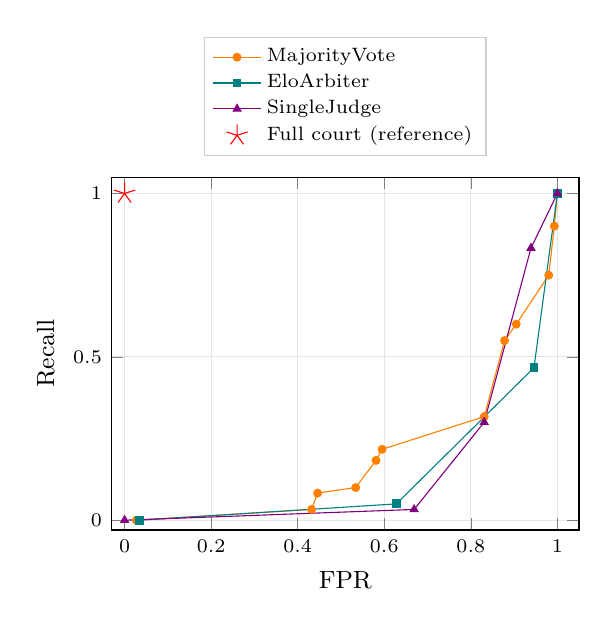
\begin{tikzpicture}
\begin{axis}[
    name=paretoplot,
    width=0.62\textwidth, height=0.5\textwidth,
    xlabel={FPR}, ylabel={Recall},
    xmin=-0.03, xmax=1.05, ymin=-0.03, ymax=1.05,
    grid=both, grid style={gray!20},
    legend to name=paretoleg,
    legend style={font=\scriptsize, draw=gray!40, row sep=-1pt,
      cells={anchor=west}},
    legend cell align=left,
    tick label style={font=\scriptsize}, label style={font=\small}]
\addplot[mark=*, mark size=1.4pt, color=orange] coordinates {
    (0.027,0.000) (0.432,0.033) (0.446,0.083) (0.534,0.100)
    (0.581,0.183) (0.595,0.217) (0.831,0.317) (0.878,0.550)
    (0.905,0.600) (0.980,0.750) (0.993,0.900) (1.000,1.000)};
\addlegendentry{MajorityVote}
\addplot[mark=square*, mark size=1.4pt, color=teal] coordinates {
    (0.034,0.000) (0.628,0.050) (0.946,0.467) (1.000,1.000)};
\addlegendentry{EloArbiter}
\addplot[mark=triangle*, mark size=1.6pt, color=violet] coordinates {
    (0.000,0.000) (0.669,0.033) (0.831,0.300) (0.939,0.833) (1.000,1.000)};
\addlegendentry{SingleJudge}
\addplot[only marks, mark=star, mark size=4pt, color=red] coordinates {(0,1)};
\addlegendentry{Full court (reference)}
\end{axis}
% 图例遮挡修复（与 fig:net 同法）：三条基线前沿贯穿整个绘图区
% （原点→(1,1)），任何轴内图例位置都会压住散点，故用 legend to
% name 生成图例后经 \node 放到轴框正上方；数据坐标零改动。
\node[anchor=south, yshift=4pt] at (paretoplot.north) {\pgfplotslegendfromname{paretoleg}};
\end{tikzpicture}
\caption{Pareto frontiers of the three aggregation baselines over the
$7\times7$ threshold grid ($t_{\mathrm{sup}}, t_{\mathrm{rej}} \in
\{0.3,\dots,0.9\}$, reject operating point), from decision-primitive
replay with zero production-code changes. The star marks the full court,
which is threshold-free by construction; no baseline grid point attains
recall $=1.0$ at FPR $=0.0$. Data:
\texttt{baseline\_sensitivity\_report.json}.}
\label{fig:pareto}
\end{figure}

\subsection{Pilot: ABP vs.\ guilty-presumption pre-screening}\label{sec:h2a}

On the full 600-case L1 layer, the guilty-presumption pre-screen (any
formal defect $\Rightarrow$ case rejection, the standard retrieval-firewall
policy) achieves recall $0.6$ at FPR $0.5$ overall—convicting 100\% of
defect-only negatives (by design) and none of the clean-neutral negatives
($0/150$), so the entire $0.5$ FPR mass sits on the defect-only half. ABP
holds recall $1.0$ / FPR $0.0$ on the same
cases. This is the empirical form of Proposition~\ref{prop:decomp}: the guilty
screen's $P(\dd)=0.203$ on the 148-case negative basis is entirely
defect-only ($S$), all of which ABP spares ($P(\mm)=0$).

\subsection{Component ablations}\label{sec:courtabl}

\begin{table}[t]
\centering\small
\caption{Court component ablation on 60$\times$2 L1 (seed 42). Conviction
layer vs.\ escalation layer. no\_abp removes the pairwise rubric (hard
constraints remain); no\_reviewer / no\_boss remove the downstream
review/override components.}
\label{tab:courtabl}
\begin{tabular}{@{}lcc|cc@{}}
\toprule
& \multicolumn{2}{c|}{Conviction} & \multicolumn{2}{c}{Escalation} \\
Mode & Recall & FPR & Recall & FPR \\
\midrule
court\_full & 1.000 & 0.000 & 1.000 & 1.000 \\
\;no\_abp & 0.000 & 0.000 & 1.000 & 1.000 \\
\;no\_reviewer & 1.000 & 0.000 & 1.000 & 1.000 \\
\;no\_boss & 1.000 & 0.000 & 0.733 & 0.800 \\
\bottomrule
\end{tabular}
\end{table}

\textbf{ABP is load-bearing}: without the pairwise rubric, conviction recall
collapses $1.0\!\to\!0.0$ (the synthetic layer contains no tool-ban
content, so the hard-constraint channel—the only remaining conviction
path—never fires). \textbf{Reviewer and BOSS are downstream of conviction}
by design: removing them leaves conviction identical (a structural
invariant asserted by red line). \textbf{BOSS is the primary escalation
signal source}: removal drops escalation recall to $0.733$ while conviction
is untouched.

\textbf{Escalation is not conviction.} On the full court, escalation FPR is
$1.0$ with precision $0.5$ (and $0.0$ on the L1.5 basis): every
defect-bearing-but-innocent case (the $S$ set of
Proposition~\ref{prop:decomp}) is \emph{routed to human review} rather than
auto-rejected. This is the intended semantics—escalation is the court's
abstention channel, and measuring precision@escalation is how the routing
budget is tuned (\S\ref{sec:casestudy} shows the complementary escalation-
type case where abstention is correct by construction).

\subsection{Scorer-level ablations}\label{sec:scorerabl}

The conviction--confidence decoupling (P2) makes a scorer ablation's
effects observable only through the confidence channel. We therefore run
two scorer ablations with the full court's switches frozen, post-processing
scores experiment-side (production code untouched), with two red-line
layers: R1 (monotonicity: ablated FPR must not exceed and recall must not
fall below full court) and R2 (effect direction: \texttt{no\_recency}
confidence must not decrease; \texttt{no\_source\_pedigree} confidence must
differ from the original—proving the ablation is live).

\begin{table}[t]
\centering\small
\caption{Scorer-level ablation (60$\times$2 L1, seed 42). avg\_pass-conf =
mean overall score of passed cases. Recall/FPR identical across rows
(decoupling invariant); the observable effect is confidence inflation.}
\label{tab:scorerabl}
\begin{tabular}{@{}lcc@{}}
\toprule
Configuration & avg.\ pass conf. & Interpretation \\
\midrule
full\_v03 (reference) & 0.4994 & calibrated baseline \\
\;no\_source\_pedigree ($s\!\to\!0.775$) & 0.5248 & low-pedigree sources lifted \\
\;no\_recency ($\to$1.0) & 0.6250 & stale evidence conflated with fresh \\
\bottomrule
\end{tabular}
\end{table}

Both red lines hold: recall/FPR are exactly $1.0/0.0$ in all rows, and the
confidence ordering quantifies each mechanism's contribution to calibration
($+0.025$ from source pedigree, $+0.126$ from recency—the largest single
effect, showing recency decay is doing most of the work in discounting
stale literature).

\subsection{Robustness: order, size, streaming, and label noise}\label{sec:robust}

\textbf{Order invariance (Proposition~\ref{prop:order}).} 1{,}000 random
permutations across 60 L1 positives, both full-court and baseline
configurations: \textbf{0} divergent verdict signatures
(invariant rate $1.0$). The court's verdicts are a function of the evidence
\emph{set}, not its order.

\textbf{Streaming ablation.} A rule-based streamed variant that terminates
on first contradiction (k=1) or first k-strong-streak (k=2) diverges from
the canonical court in $70/1000=0.070$ permutations (k=1; 10/60 cases
affected; permuted recall aggregated over all case--permutation
evaluations $0.924$ vs.\ the same variant's canonical-order recall $0.95$
on the 60 positives, court canonical $1.0$) and $2/1000=0.002$ (k=2,
recall $0.998$). Order sensitivity is real
for early-termination designs and decays as the termination threshold
tightens—supporting the design choice of full deliberation before
disposition.

\textbf{Counting-law calibration (Theorem~\ref{thm:counting}).} Under
controlled null cases ($p_0=0.30$ designed defect injection, unique-source
construction so that all $\binom{m}{2}$ pairs are live, 300 trials per
$m\in\{3,5,10,20\}$): the log-log slope of false pairs against
$\binom{m}{2}$ is $0.942$ (expected $1.0$), and the advantage ratio
$\rho(m)=\bar D/\bar K$—guilty-screen defect budget $\bar D$ over ABP
false-pair budget $\bar K$—decays against $(m-1)$ with log-log slope
$-0.857$ (expected $-1.0$), matching the counting law's $1/(m-1)$
scaling; the empirical ratio coincides with the Bonferroni form at every
grid point (ratio/bound $=1.0$), and the budgets intersect at crossover
$m^\ast\!\approx\!18.5$. The court's counting advantage is therefore
concentrated in small-to-moderate cases and erodes with case size, exactly
as the counting law predicts (the crossover figure is for the ungated
baseline rubric; the gates cut $q_K$ $6$--$13\times$
(\S\ref{sec:decomp}), pushing the full court's crossover well beyond the
scanned range).

\textbf{Source-label noise ($\pm 20\%$).} A corruption pass re-labels
exactly $\max(1, \lfloor 0.2m \rceil)$ sources per case (50 replicates per
case; only \texttt{source} fields change, with field-level oracle
invariants asserted). On 7{,}400 negative replicates (L1 + L1.5),
\textbf{zero} false convictions are induced—the only theoretical attack
(un-ignoring a same-source skipped pair) has no fuel on these bases, and
the red line treats this claim as falsifiable: any induced case would be
written to an audit field with its pair endpoints (observed: empty). On
3{,}000 positive replicates, 62 convictions are lost ($2.07\%$; the sole
channel is a core pair re-labelled same-source), leaving noisy recall
$0.9793$; pair-set flip rate $13.9\%$, intensity flip $14.1\%$, mean
$|\Delta\text{conf}|$ $0.0076$ (max $0.578$, attained when all pairs are
simultaneously suppressed). The positive-loss asymmetry is reported, not
red-lined: it is a directional finding, not a defect.

\subsection{Network-failure discrimination}\label{sec:network}

Citation verifiers call network APIs; verification outages are routine. The
community-standard \textbf{two-state} policy (\texttt{valid} vs.\ ``anything
else'') conflates ``could not verify'' with ``fabricated.'' Our production
\textbf{three-state} policy maps \texttt{network\_failed} to a warning that
cannot convict, with 3$\times$ exponential-backoff retries and a cross-case
TTL cache. We inject deterministic transport failures
(\texttt{httpx.MockTransport}) at rates $p\in\{0, 0.3, 0.5, 1.0\}$ over 60
clean-claim cases (all references valid, shared 40-hot-PMID pool) and 20
invalid-reference cases (recall control). Both policies consume the
identical production verification/retry/cache stack; the only variable is
the failure-mapping policy.

\begin{table}[t]
\centering\small
\caption{Network-failure experiment (Fig.~\ref{fig:net}): FPR on clean
claims / recall on invalid-reference claims, by policy and failure rate
$p$.}
\label{tab:network}
\begin{tabular}{@{}lcccc@{}}
\toprule
& $p=0$ & $p=0.3$ & $p=0.5$ & $p=1.0$ \\
\midrule
Three-state FPR (clean) & \textbf{0.000} & \textbf{0.000} & \textbf{0.000} & \textbf{0.000} \\
Two-state FPR (clean) & 0.000 & 0.667 & 0.833 & 1.000 \\
Three-state recall (invalid) & 1.000 & 1.000 & 0.900 & 0.000$^{\dagger}$ \\
Two-state recall (invalid) & 1.000 & 1.000 & 1.000 & 1.000 \\
\bottomrule
\end{tabular}
\\[2pt]
{\footnotesize $^{\dagger}$At full outage the three-state court abstains on
all cases (refuses to adjudicate rather than guessing)—consistent with the
presumption-of-innocence principle; the two-state policy's ``perfect
recall'' is purchased entirely with clean-claim false positives.}
\end{table}

\begin{figure}[t]
\centering
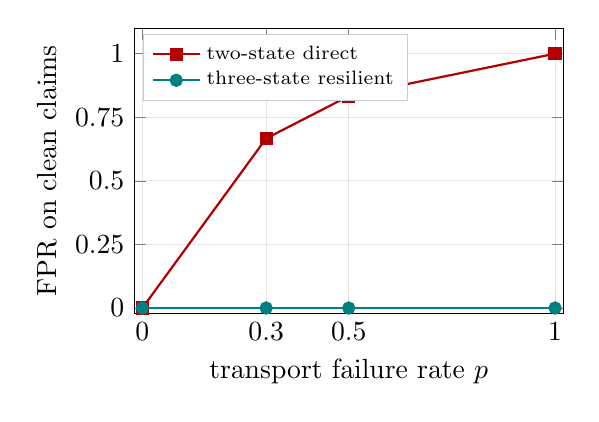
\begin{tikzpicture}
\begin{axis}[
  width=0.58\textwidth, height=5.2cm,
    xlabel={transport failure rate $p$},
    ylabel={FPR on clean claims},
    xmin=-0.02, xmax=1.02, ymin=-0.02, ymax=1.1,
    xtick={0,0.3,0.5,1.0}, ytick={0,0.25,0.5,0.75,1.0},
    legend style={at={(rel axis cs:0.02,0.98)}, anchor=north west,
      font=\scriptsize, draw=gray!40, row sep=-1pt,
      cells={anchor=west}},
  legend cell align=left,
  grid=both, grid style={gray!20},
]
\addplot[color=red!70!black, thick, mark=square*] coordinates {(0,0) (0.3,0.6667) (0.5,0.8333) (1.0,1.0)};
\addlegendentry{two-state direct}
\addplot[color=teal, thick, mark=*] coordinates {(0,0) (0.3,0) (0.5,0) (1.0,0)};
\addlegendentry{three-state resilient}
\end{axis}
\end{tikzpicture}
\caption{Clean-claim false-positive rate under injected citation-verification
failures. The two-state policy's FPR is monotone in $p$ and reaches $1.0$ at
full outage; the three-state policy is structurally flat at $0$ (network
failures cannot enter the conviction channel). Data: Table~\ref{tab:network};
source report \texttt{backend/tests/ddb/network\_failure\_report.json}.}
\label{fig:net}
\end{figure}

Process metrics confirm the mechanisms: the three-state policy's mean
attempts rise $1.00\!\to\!1.33\!\to\!1.75\!\to\!3.00$ with $p$ (retry effect
observable), and the cross-case cache absorbs $133$ lookups (shared-pool
reuse), cutting transport requests at $p=0.3$ from $212$ to $103$. Six
pre-registered red lines pass, including bit-exact determinism of a
double-run at $p=0.5$.

\textbf{Relation to abstention-aware evaluation.} The three-state policy
instantiates the same design stance as abstention-aware evaluation in
scientific citation generation, where hallucination-rate-centred metrics
dominate \citep{saxena2024reasons}: uncertainty should yield an explicit
non-committal outcome, not a conviction. The contribution here is
orthogonal—citation-generation abstention metrics measure generation-side
behaviour, whereas Table~\ref{tab:network} quantifies the downstream
adjudication cost of omitting the third state, as a function of the
transport failure rate.

\subsection{Advantage-decomposition calibration}\label{sec:decomp}

On the 148-case negative basis (Table~\ref{tab:decomp}; $\cset=\emptyset$;
60 L1 negatives of which
30 defect-only, plus 88 L1.5 pseudo-conflicts), with the real pre-screen as
the $\dd$ labeler and the real ABP rubric as the $\mm$ labeler:

\begin{table}[t]
\centering\small
\caption{Proposition~\ref{prop:decomp} calibration. Cell counts and closure of
$\Pr(\dd)-\Pr(\mm)=\Pr(S)-\Pr(M{\setminus}\dd)$ on the negative basis.}
\label{tab:decomp}
\begin{tabular}{@{}lccccc@{}}
\toprule
Config & $P(\dd)$ & $P(\mm)$ & $\Pr(S)$ & $\Pr(M{\setminus}\dd)$ & residual \\
\midrule
full\_v03 & 0.2027 & 0.0000 & 0.2027 & 0.0000 & $\mathbf{0}$ \\
baseline\_v02 & 0.2027 & 0.5946 & 0.2027 & 0.5946 & $\mathbf{0}$ \\
\bottomrule
\end{tabular}
\end{table}

The identity holds \emph{by construction} (residual $0$, tolerance
$10^{-12}$, for both configurations—this is expected, since the identity is
a set-algebra proposition, not an empirical finding); the empirical content
is the pure layer attribution: all $S$ cases
(30/30) come from L1 defect-only; all $M{\setminus}\dd$ (88/88 under
baseline switches) come from L1.5 pseudo-conflicts—each benchmark family
measures exactly the channel it was built for.

\textbf{Dependency calibration.} On controlled null cases ($m=20$, 300
trials, 57{,}000 pair opportunities per configuration): baseline
$q_K=0.0355$ vs.\ full $q_K=0.0058$ (the gates cut per-pair mismatch rates
$6$--$13\times$); adjacent-pair joint events yield $\kappa=1.42$ (baseline)
and $2.47$ (full), both above the $\kappa\geq1$ independence line
(stronger dependence in the full court is expected—gates induce
correlated suppression), with joint-event counts ($1{,}829$ / $86$)
adequate for estimation.

\subsection{Role-weight calibration}\label{sec:roles}

The 13 agent roles' evidence weights (Appendix~\ref{app:roles}) were
calibrated by single-role perturbation over a 208-case pool (L1 60$\times$2
+ L1.5), for both arbitration arbiters that consume role weights. Red
lines: coverage $\geq5$ cases/role (achieved 27--55), positive control
($\times0.1$ perturbation) must flip $\geq1$ decision (achieved 7/6/6 flips
on pi-agent/drug-researcher/report-expert—proving the pipeline is live),
and decision flip rate $\leq0.05$ at $\pm20\%$.

Observed maximum flip rate: $4/208=0.0192$ (data-specialist at
$\times0.8$, identical for both arbiters)—the maximum occurs in the
down-weight direction, while up-weight perturbations also flip a small
number of decisions (at most $2/208$ per role at $\times1.2$, identical
for both arbiters); every rate is far below the $0.05$ line. Verdicts are
driven by contradiction structure, not by weight tuning: the role table is
a calibration surface, not a decision surface.

\subsection{End-to-end case studies on real literature disputes}\label{sec:casestudy}

Two L2 disputes, run through the full seven-step court with full
intermediate-state logging (timeline, ABP pair ledger with intensities,
per-evidence scores, filtered-evidence audit, verdict chain):

\textbf{Deadlock type (DDB-L2-0001): EGFR triple-mutation inhibition.}
Both sides carry top-venue evidence (allosteric route: Nature 2016
\citep{jia2016eai045} / Cancer Lett 2017 \citep{wang2017eai045};
ATP-covalent route: NEJM FLAURA/OS
\citep{soria2018osimertinib,ramalingam2020os}). Zero evidence is filtered;
ABP detects the gold contradiction pair (L2-01-EV-02 $\times$ L2-01-EV-03,
intensity 3), the case is convicted, and the PI arbitrates \emph{conditional
support} at confidence $0.528$; four escalation clauses fire (low
confidence, conditional-support policy, reviewer objection, intensity-3
mandatory review). This is the ``both sides are credible'' regime in which
vote-style aggregation degenerates: the court produces a traceable chain
from detected pair to human-review routing.

\textbf{Escalation type (DDB-L2-0005): AF3 complex-prediction dispute.}
Every evidence item cites AlphaFold2/3, hitting the platform's
structure-prediction tool ban; the symmetric pre-screen filters all
evidence; the court finds itself with no adjudicable evidence, abstains
(decision \emph{unable to adjudicate}, confidence $0.0$), and escalates the
entire case to human review. Gold-pair detection is not applicable in this
regime—the gap between the two cases' regimes is itself a finding: the
court distinguishes ``conflict to resolve'' from ``nothing to judge,''
and refuses to fabricate a verdict in the latter.

\textbf{Honesty note.} Grounded in verified real literature, these case
studies are \emph{not} production-platform runs; the outline's
envisioned ``5-round group-chat deadlock'' narrative segment is replaced,
faithfully, by the seven-step court timeline, and production-run case
studies (ASFV and canine vaccine pipelines, \S\ref{sec:limits}) remain
pending until the L3 layer is built.

% -------------------------------------------------------------------------
\subsection{Executed LLM-side ablations}\label{sec:llmablation}

The two ablations registered as pending in the research plan---swapping the
rule-based PI arbiter for a hosted LLM, and running a PROClaim/DebateCV-style
prosecution--skeptic--judge debate verifier on identical evidence
pools---have now been executed against a hosted LLM
(\texttt{qwen-flash}, temperature~0; configuration and commands in
Appendix~\ref{app:repro}). Both are evaluated on the same 208-case pool as
Table~\ref{tab:main} (60 positives, 148 negatives), with the court's
outputs \emph{frozen in advance} from the pre-registered baseline report,
under the identical reject and non-support operating points. Evidence is
presented blind: \verb|evidence_id|, \verb|source|, \verb|role|,
\verb|content| only---no scores, no gold labels, no court verdicts.
Table~\ref{tab:llmabl} reports the outcome, taken verbatim from
\texttt{llm\_arbiter\_report.json} and \texttt{llm\_debate\_report.json}.

\begin{table}[t]
\centering\small
\begin{tabular}{@{}lcccc@{}}
\toprule
System & Recall $\uparrow$ & 95\% CI & FPR $\downarrow$ & 95\% CI \\
\midrule
\multicolumn{5}{@{}l}{\textit{Court (frozen reference, rule-based PI arbiter)}}\\
\court{} & $1.000$ & $[0.940, 1.000]$ & $0.000$ & $[0.000, 0.025]$ \\
\midrule
\multicolumn{5}{@{}l}{\textit{LLM arbiter (208 cases, 0 unresolved failures)}}\\
LLM arbiter & $0.983$ & $[0.911, 0.997]$ & $0.500$ & $[0.421, 0.580]$ \\
\midrule
\multicolumn{5}{@{}l}{\textit{LLM debate (208 cases $\times$ 3 roles, 0 unresolved failures)}}\\
LLM debate & $0.700$ & $[0.575, 0.801]$ & $0.372$ & $[0.298, 0.452]$ \\
\bottomrule
\end{tabular}
\caption{Executed LLM-side ablations on the 208-case pool (reject
operating point; positive class = case contains a true contradiction).
The court row is frozen from the pre-registered baseline comparison; the
two LLM rows are executed results with resume-for-missing-calls (each case
retains its first successful response; single model, one protocol round
per case). Sensitivity (non-support) operating points, per-verdict
distributions, and call-failure accounting are in the accompanying JSON
reports.}
\label{tab:llmabl}
\end{table}

Three observations, reported regardless of direction. \textbf{(1) Recall is
not what separates the rule core from LLM arbitration.} The single-LLM
arbiter reaches $0.983$ recall---within one positive case of the court's
$1.0$---because on this synthetic benchmark outright contradictions are
linguistically conspicuous. \textbf{(2) The separation is entirely in the
false-conviction dimension.} The LLM arbiter convicts
$\mathrm{FPR}=0.500$ [0.421, 0.580] of the 148 well-formed negatives while
the court convicts none (FPR~$0.000$, CI upper bound $0.025$); on the
non-support operating point the arbiter convicts $0.980$ of negatives
(accuracy $0.303$). The asymmetric burden of proof---not rhetorical
competence---is what keeps benign evidence out of the conviction column,
which is precisely the paper's central claim measured on the LLM's
home turf. \textbf{(3) Adding adversarial structure without a conviction
rule does not help.} The 3-call debate protocol \emph{degrades} relative
to single-shot arbitration (recall $0.700$ vs.\ $0.983$; $\Delta
\text{recall}=-0.300$ vs.\ the frozen court) and never supports a
well-formed claim (0 support verdicts out of 208---consistent with the
prosecution's framing prevailing over the skeptic's across both
polarities, as judged by the final verdict distribution), while still
convicting
$0.372$ of negatives. Structured LLM argumentation inherits the same
false-conviction failure mode that motivates the court's presumption of
innocence, and the debate framing adds no mechanism to bound it.

\textbf{Honesty note.} These runs are exploratory rather than tuned: one
hosted model at temperature~0, one round each, no prompt ensembling.
A pre-registered configuration deviation is declared: the planned
\texttt{max\_tokens}=300 was raised to 2048 because the hosted
\texttt{qwen-flash} gateway enables chain-of-thought by default and the
300-token budget was exhausted by reasoning tokens, leaving the verdict
payload empty; the deviation and its reason are recorded in the reports'
\texttt{max\_tokens\_deviation} fields. Structural red lines all hold
(complete response coverage, verdict-enum integrity with raw-response
re-parsing, frozen court reference match); conservative handling of
unresolved cases (not-caught under reject, caught under non-support) is
declared in the reports' \verb|prediction_mapping| fields. Results
follow the same pre-registration discipline as the deterministic
experiments and are excluded from the zero-LLM regression.

% -------------------------------------------------------------------------
\section{Discussion}\label{sec:discussion}

\textbf{Why courtroom procedure, not voting.} The baseline failures in
Table~\ref{tab:main} are not implementation artefacts but category errors:
majority voting aggregates \emph{preferences}, while scientific arbitration
must aggregate \emph{evidence under a burden of proof}. Once conviction
requires a contradiction pair, the system's recall/FPR profile is governed
by detection quality (gates, aspects, intensity) rather than by vote
thresholds—and every detection component is individually ablatable
(Tables~\ref{tab:courtabl}--\ref{tab:scorerabl}) with red-line-guarded
attribution.

\textbf{Escalation as a first-class outcome.} The escalation layer's
apparently poor ``precision'' ($0.5$ on smoke sets, $0.0$ on the negative
basis) is the design working as intended: the $S$ set of
Proposition~\ref{prop:decomp}—defect-bearing, contradiction-free, therefore
innocent—\emph{must} be routed to humans rather than auto-rejected. The
operational question is routing budget, not escalation FPR; the deadlock /
escalation case-study pair (\S\ref{sec:casestudy}) illustrates both regimes.

\textbf{An escalation cost model.} The routing question can be made
falsifiable. Let $c$ be the cost of one human review, $L$ the loss incurred
by one wrongful automatic rejection of an innocent claim,
$N_{\mathrm{esc}}$ the number of escalated cases, and $\hat p$ the
precision@escalation. The escalate-over-error policy costs
$C_{\mathrm{esc}} = c\,N_{\mathrm{esc}}$; an auto-reject policy that
dismisses exactly the escalated set costs
$C_{\mathrm{auto}} = (1-\hat p)\,L\,N_{\mathrm{esc}}$. Escalation is the
cheaper policy if and only if $c/L < 1-\hat p$. On the 148-case negative
basis (\S\ref{sec:decomp}), every escalated case is innocent
($\hat p = 0$), so escalation dominates for any $c < L$: one wrongful
auto-rejection must cost more than one review. On the 60$\times$2 L1 smoke
set (\S\ref{sec:courtabl}), $\hat p = 0.5$, so escalation dominates iff
$c < L/2$. The model turns the P3 principle from a design stance into a
testable proposition: any deployment reporting precision@escalation and
review cost can read off the cheaper channel, and the red-line-guarded
precision measurements (\S\ref{sec:courtabl}, \S\ref{sec:decomp}) supply
the measured inputs.

\textbf{Infrastructure failures are a scientific-validity concern.}
Table~\ref{tab:network} shows that a standard engineering default (fail
closed) translates directly into convicting up to $100\%$ of clean claims
during outages. A three-state evidentiary policy costs nothing at $p=0$,
preserves most recall at moderate $p$ through retries and caching, and
abstains rather than fabricates at full outage. We suggest that any
verifier-gated adjudication system report its failure-mode FPR curve
alongside its clean-condition accuracy.

\textbf{ABP and LLMs are complementary, not competing.} A common
misreading of the zero-LLM discipline is that \court{} rejects LLM
integration. The opposite is true: ABP is a \emph{procedural architecture}
structurally decoupled from the arbitration substrate, and LLMs can occupy
any of three slots inside it. (i)~As the \emph{scorer}: an LLM can replace
the rule-based source-pedigree/relevance scorer (Eq.~\ref{eq:overall}); by
the P2 decoupling invariant this changes confidence calibration but cannot
move recall or FPR. (ii)~As the \emph{contradiction detector}: an LLM can
enrich the aspect-matching and intensity-grading that feed ABP conviction,
potentially raising recall on semantically non-obvious disputes. (iii)~As
the \emph{arbiter}: an LLM can replace the PI-agent in step~4 of
\S\ref{sec:court}; \S\ref{sec:llmablation} tests this slot \emph{without}
ABP and finds FPR $0.500$, which is precisely why the ABP conviction rule
must be retained regardless of arbiter choice. The target production
architecture is therefore \emph{LLM components inside an ABP envelope},
not LLM-as-verifier without procedural guardrails; the zero-LLM core
experiments isolate the envelope's contribution, and the LLM ablations
quantify what happens when the envelope is removed.

% -------------------------------------------------------------------------
\section{Limitations}\label{sec:limits}

We state the boundaries of the present evidence explicitly.

\begin{enumerate}[leftmargin=2em,itemsep=2pt]
\item \textbf{No user study yet.} The planned 10-participant blind A/B
evaluation (SUS trust, NASA-TLX workload, open feedback vs.\ Elo and
single-judge outputs) has not been run; all claims here concern system
behaviour, not user experience.
\item \textbf{No production-run (L3) layer.} \ddb{}'s L3 layer—claims,
evidence, and verdicts harvested from real platform runs, including the
group-chat deadlock narratives and wet-lab action orders—does not exist
yet. The case studies (\S\ref{sec:casestudy}) use verified real literature
but are benchmark-grounded, not production logs.
\item \textbf{LLM-side ablations: partial.} Two of the registered LLM-side
ablations have now been executed against a hosted LLM (qwen-flash,
temperature 0): the LLM-arbiter ablation (swapping the rule-based PI
arbiter for a direct LLM three-verdict arbiter) and a protocol-level
LLM-debate verifier following the PROClaim \citep{chowdhury2026proclaim}
and DebateCV \citep{he2026debatecv} prosecution--skeptic--judge structure,
both consuming identical evidence pools with the court's outputs frozen in
advance and evaluation under the same reject/non-support operating points
of Table~\ref{tab:main} (\S\ref{sec:llmablation}). The third registered
ablation—replacing the position-weight proxy with LLM-based structural
role annotation—remains pending, as does head-to-head evaluation against
the third-party verifier systems themselves; the protocol-level comparison
reported here uses our own debate prompts rather than the systems'
trained pipelines.
\item \textbf{L2 scale and annotation status.} The L2 layer is 10 cases
(target 45+), all positives (FPR-relevant neutral sets are a second-batch
item), and expert adjudication is pending; gold pairs are construction-time
annotations, and keyword-channel sensitivity means ABP's L2 conclusions
must eventually be cross-validated with expert and LLM-judge channels. The
expansion protocol is already designed: grow L2 to at least 45 cases
including a neutral negative family (target FPR $=0$ under the same
gate-purity red line as L1.5), have every case annotated by three domain
experts under the dual-track protocol (three experts plus an independent
evidence-verification track), and report Krippendorff's $\alpha$ even if
low, following \citealp{cecil2026beyond}; the pre-registered acceptance
red line is that ABP recall on expert-adjudicated L2 must stay within the
Wilson interval reported in \S\ref{sec:ddb}. Results below that bound
would falsify the generalisation claim and will be reported as such.
\item \textbf{Third-party benchmark cross-validation.} All current
benchmark layers are author-built. The next cycle adds a cross-validation
arm on at least one independently constructed claim-verification benchmark,
with the court and the strongest baseline evaluated under identical
splits, prompts (where applicable), and operating points; divergence
between author-built and third-party results will be analysed and reported
regardless of direction. This arm is designed but not yet executed, and no
third-party numbers appear in this paper.
\item \textbf{Negative-set composition bias.} The L1 negative half is
composed of defect-bearing (150 defect-only) and clean-neutral (150) cases
by construction. This composition structurally favours the court on the
defect-sensitivity axis measured by the guilty-presumption pilot
(\S\ref{sec:h2a}) and biases score-driven baselines that reward evidence
quality; the baseline gaps reported here should be read as measuring this
design axis, not as a universal baseline deficit, pending the third-party
cross-validation arm above.
\item \textbf{Protection relies on cross-source disagreement.} The ABP
pair channel convicts only on cross-source contradiction pairs: same-source
pairs are skipped by the gate, so a contradiction internal to a single
source is outside the pair channel's scope and falls to the hard-constraint
channel or to escalation. Domains where opposing evidence routinely shares
a single source therefore retain less of the court's protective margin.
\item \textbf{Smoke-scale statistics.} Reported experiments run at
regression scale (60--300 cases per cell) for determinism and CI cost; the
pre-registered main experiment (600$\times$2 full-combinatorial ablations
with significance tests) runs on the same pipelines at scale.
\item \textbf{Zero-LLM scope.} The main benchmark, all baselines, and all
red-line experiments are deterministic rule systems; the two LLM-side
ablations of \S\ref{sec:llmablation} are the only pipelines that invoke an
LLM, and the production platform's LLM components (evidence authoring,
group-chat debate) remain upstream and unevaluated here.
\end{enumerate}

% -------------------------------------------------------------------------
\section{Conclusion}\label{sec:conclusion}

\court{} reframes evidence aggregation in multi-agent research pipelines as
procedural arbitration: presume innocence, convict only on detected
contradiction structure, score for calibrated confidence, escalate what
cannot be judged, and never let infrastructure failures impersonate
scientific findings. Three results carry the evidential weight and do not
depend on the benchmark's hand-adjudicated gold labels: the counting law's
calibrated advantage profile (slopes $0.942$/$-0.857$ against expected
$1.0$/$-1.0$, with the empirical ratio coinciding with the Bonferroni form
at every grid point and the advantage concentrated in small-to-moderate
cases), the three-state verification policy's zero network-failure false
positives under matched injection---abstaining at full outage rather than
fabricating---and the conviction--confidence decoupling invariant preserved
under every scorer ablation. On the author-built synthetic layer of the
954-case benchmark (evaluation at regression scale, \S\ref{sec:limits}),
the full court is the only system that holds recall $1.0$ / FPR $0.0$
against all three standard aggregation baselines at every threshold
setting scanned, and its verdicts are permutation-invariant. Every number
from the deterministic pipelines is produced under pre-registered red
lines wired into CI, and the two executed LLM-side ablations report their
hosted-LLM results against the same frozen operating points
(\S\ref{sec:llmablation}). The path to a complete preprint runs through the
pending items above: expansion and expert adjudication of L2, third-party
benchmark cross-validation and third-party head-to-head verifier
evaluation, the L3 production layer, the user study, and the LLM-based
structural role annotation ablation—each is a bounded, scripted increment
on infrastructure that already exists.

% -------------------------------------------------------------------------
\bibliographystyle{unsrtnat}
\bibliography{references}

\appendix

% -------------------------------------------------------------------------
\section{Agent role evidence-weight registry}\label{app:roles}

Evidence-credibility weights used by both arbiters (registered per role;
unregistered roles fall back to $0.5$; the platform's
\texttt{data-analyst} implements the paper's \texttt{data-specialist}
profile, with the platform-side fallback difference disclosed in the
project's role-profile appendix):

\begin{table}[h]
\centering\small
\begin{tabular}{@{}llll@{}}
\toprule
Role & Weight & Role & Weight \\
\midrule
pi-agent & 1.0 & data-specialist & 0.75 \\
drug-researcher & 0.9 & qc-inspector & 0.7 \\
structural-biologist & 0.9 & knowledge-engineer & 0.65 \\
computational-chemist & 0.85 & reflexion-agent & 0.6 \\
synthetic-chemist & 0.8 & project-coordinator & 0.6 \\
antibody-engineer & 0.8 & report-expert & 0.5 \\
peptide-designer & 0.75 & & \\
\bottomrule
\end{tabular}
\end{table}

Design principles: first-hand evidence $>$ computational
heuristics $>$ organisational/expressive cues; adjacent gap $\geq 0.05$.

% -------------------------------------------------------------------------
\section{Escalation clauses}\label{app:clauses}

The escalation decision is the disjunction of: (1) any reviewer objection;
(2) PI confidence below the conditional-support threshold; (3) dual-track
divergence between the rule-arbitration track and the evidence-review
track; (4) decision in a policy-mandated review category; (5) any
intensity-3 convicted contradiction pair (mandatory human review); (6)
insufficient adjudicable evidence (abstention). Clauses 4 and 6 are what
make the escalation-type case study (\S\ref{sec:casestudy}) behave as it
does: a fully filtered case cannot be convicted \emph{or} acquitted, so it
must be escalated.

% -------------------------------------------------------------------------
\section{Pre-registered red lines (summary)}\label{app:redlines}

Each experiment family ships with machine-checked red lines, each paired
with an anti-test that fabricates a violation to prove the checker is live:
baseline comparison (court strictly dominates all three baselines on both
operating points); component ablation (no\_abp conviction collapse on L1;
reviewer/BOSS conviction invariance; BOSS escalation monotonicity; headless
pipeline parity with production \texttt{hold\_court}); scorer ablation
(R1 monotonicity; R2 effect direction); robustness (permutation
divergence $=0$; counting-law slopes within bands; noise-induced negative
convictions $=0$ with audited empty set; noise recall $\geq 0.95$; mean
$|\Delta$conf$| \leq 0.05$); advantage decomposition (exact closure;
zero critical evidence; $P(S) > P(M{\setminus}\dd)$; $q_K$ ordering;
$\kappa\geq1$); network failure (three-state FPR $\equiv 0$; recall
profile; two-state monotone pollution curve; two-state recall
invariance; bit-exact double-run; cache effect); role calibration
(coverage, positive control, flip rate).

% -------------------------------------------------------------------------
\section{Reproducibility}\label{app:repro}

All experiments run from a single regression entry point, the bash script
\texttt{backend/tests/scripts/} \linebreak
\texttt{run\_v03\_regression.sh}, with
deterministic seed 42 and no network or LLM calls (the network-failure
experiment's failures are injected at the transport layer). The two
LLM-side ablations of \S\ref{sec:llmablation} run outside this regression
via a dedicated entry point and require network access to a hosted LLM
endpoint. Per-experiment commands and report files (last two rows: network
required):

\begin{table}[h]
\centering
\setlength{\tabcolsep}{3pt}
\scriptsize
\begin{tabular}{@{}lll@{}}
\toprule
Experiment & Script & Report \\
\midrule
Main comparison & \texttt{run\_baseline\_comparison.py} & \texttt{baseline\_comparison\_report.json} \\
Threshold sensitivity & \texttt{run\_baseline\_sensitivity.py} & \texttt{baseline\_sensitivity\_report.json} \\
Component ablation & \texttt{run\_ablation\_v03.py -{}-court} & \texttt{ablation\_v03\_report.json} \\
Scorer ablation & \texttt{run\_ablation\_v03.py -{}-scorer-ablation} & \texttt{ablation\_v03\_report.json} \\
Robustness A--D & \texttt{run\_robustness\_experiments.py} & \texttt{robustness\_report.json} \\
Decomposition & \texttt{run\_advantage\_decomposition.py} &
\texttt{advantage\_decomposition\_report.json} \\
Role calibration & \texttt{run\_role\_weight\_calibration.py} & \texttt{role\_weight\_calibration.json} \\
Network failure & \texttt{run\_network\_failure\_experiment.py} & \texttt{network\_failure\_report.json} \\
Case studies & \texttt{run\_case\_study.py} & \texttt{case\_study\_report.json} \\
H2a pilot & \texttt{pilot scripts (backend/tests/scripts)} & \texttt{pilot\_h2a\_report.json} \\
LLM arbiter ablation & \texttt{run\_llm\_arbiter\_experiment.py} & \texttt{llm\_arbiter\_report.json} \\
LLM debate (protocol-level) & \texttt{run\_llm\_debate\_experiment.py} & \texttt{llm\_debate\_report.json} \\
\bottomrule
\end{tabular}
\end{table}

The last two rows require network access to a hosted LLM (config via
\texttt{LLM\_EXPERIMENT\_*} environment variables; model \texttt{qwen-flash},
temperature 0) and are excluded from the zero-LLM regression.

\Ddb{} layer files: \texttt{backend/tests/ddb/\{l1,l15,l2,l4\}\_cases.json}, each
locked to its generator by deep-equality consistency tests.

\end{document}
